\documentclass{article}

\usepackage{ipprocess}
%\usepackage{lmodern}
%\usepackage{longtable}
\usepackage[latin1]{inputenc} 
\usepackage[T1]{fontenc}
\pagestyle{fancy}
\usepackage{libertine}

%\usepackage[author={Jo�o Carlos Nunes Bittencourt}]{pdfcomment}

\sloppy

\title{32-bit uDLX Core Processor}

\graphicspath{{./pictures/}} % Diret�rio padr�o de figuras.
\makeindex
\begin{document}
  \capa{1.0}{abril}{2014}{32-bit uDLX Core Processor}{System Specification}{Universidade Federal da Bahia}
  \newpage

%%%%%%%%%%%%%%%%%%%%%%%%%%%%%%%%%%%%%%%%%%%%%%%%%%
%% GNU LGPL Licence
%%%%%%%%%%%%%%%%%%%%%%%%%%%%%%%%%%%%%%%%%%%%%%%%%%

  
\begin{center}
\begin{Large}\textbf{GNU LGPL License}                          \end{Large}
\end{center}
\vspace{2cm}
\fbox{
  \parbox{.7\textwidth}{
    \vspace{0,5cm}
    \begin{scriptsize}
    This file is part of uDLX (micro-DeLuX) soft IP-core.\\

    uDLX is free soft IP-core: you can redistribute it and/or modify
    it under the terms of the GNU General Public License as published by
    the Free Software Foundation, either version 3 of the License, or
    (at your option) any later version.\\

    uDLX soft core is distributed in the hope that it will be useful,
    but WITHOUT ANY WARRANTY; without even the implied warranty of
    MERCHANTABILITY or FITNESS FOR A PARTICULAR PURPOSE. See the
    GNU General Public License for more details.

    You should have received a copy of the GNU General Public License
    along with uDLX. If not, see <http://www.gnu.org/licenses/>.
    \end{scriptsize}
    \vspace{0,5cm}
  }
}

\newpage

%%%%%%%%%%%%%%%%%%%%%%%%%%%%%%%%%%%%%%%%%%%%%%%%%%
%% Hist�rico de Revis�es
%%%%%%%%%%%%%%%%%%%%%%%%%%%%%%%%%%%%%%%%%%%%%%%%%%
  \section*{\center Hist�rico de Revis�es}
  \vspace*{1cm}
  \begin{table}[ht] % aqui come�a o ambiente tabela
  \centering
  \begin{tabular}[pos]{|m{2cm} | m{7.2cm} | m{3.8cm}|} 
  \hline % este comando coloca uma linha na tabela
  \cellcolor[gray]{0.9}
  \textbf{Date} & \cellcolor[gray]{0.9}\textbf{Description} & \cellcolor[gray]{0.9}\textbf{Author(s)}\\ \hline
  \hline
  \small 04/14/2014 & \small Conception & \small Jo�o Carlos Bittencourt \\ \hline
  \end{tabular}
  \label{tab:revisoes}
  \end{table}
  
  \newpage
  
  \tableofcontents
  \newpage

%%%%%%%%%%%%%%%%%%%%%%%%%%%%%%%%%%%%%%%%%%%%%%%%%%
%% Concent
%%%%%%%%%%%%%%%%%%%%%%%%%%%%%%%%%%%%%%%%%%%%%%%%%%
  \section{Introduction}
  \subsection{Purpose}
  The main purpose of this document is to define specifications of a uDLX implementation and to provide a full overview of the design. This specifications defines all implementation parameters that composes the general uDLX requirements and specification. This definitions include processor operation modes, instruction set (ISA) and internal registers characteristics. This document also include detailed information of pipeline stages architecture, buses and other supplemental units.
  
  \subsection{Document Outline Description}
  This document is outlined as follow:
	
	\begin{itemize}
	  \item Section : 
	  \item Section : 
	\end{itemize}
		
  \subsection{Acronyms and Abbreviations}
  Along this and other documents part of this project, it will be recurrent the usage of some acronyms and abbreviations. In order to keep track of this elements the Table \ref{tab:definitions} presents a set of abbreviations used and its corresponding meaning.
  
  \FloatBarrier
  \begin{table}[H] % aqui come�a o ambiente tabela
    \begin{center}
      \caption{Acronym and descriptions of elements in this document.}
      \label{tab:definitions}

      \begin{tabular}[pos]{|m{2cm} | m{8cm}|} 
	\hline % este comando coloca uma linha na tabela
	\cellcolor[gray]{0.9}\textbf{Acronym} & \cellcolor[gray]{0.9}\textbf{Description} \\ \hline
	RISC & Reduced Instruction Set Computer \\ \hline
	GPR & General Purpose Registers \\ \hline
	FPGA & Field Gate Programmable Array \\ \hline
	GPPU & General Purpose Processing Unit \\ \hline
	SDRAM & \\ \hline
	HDL & Hardware Description Language \\ \hline
	RAW & Read After Write \\ \hline
	CPU & Central Processing Unit \\ \hline
	ISA & Instruction Set Architecture \\ \hline
	ALU & Arithmetic and Logic Unit \\ \hline
	PC  & Program Counter \\ \hline
	RFlags & Flags Register \\ \hline
	Const  & Constant \\ \hline
      \end{tabular}
    \end{center}
  \end{table}
  
  \subsection{Overview}
  The uDLX (said micro-DeLuX) is a 32-bit simple RISC-type architecture. It features a minimal instruction set, relatively few addressing modes, and a processor organization designed to simplify implementation. Its architecture was designed to be reusable and the implementation strategy was based on incremental improvements in order to produce several designs.

  The uDLX hardware structure has a five-deep pipeline architecture, and was highly designed to cover mid-low complexity applications. The uDLX is a 32-bit word- oriented system. Its architecture has 16 GPR (General Purpose Registers) in a register file. Two of these registers are reserved for special purposes. Register 0 always contains zero. It can be used as a source operand whenever zero is needed, and stores to it have no effect. Register 31 is reserved for use by some uDLX instructions, as will be described shortly. uDLX also has a 32 bit program counter.
  
  uDLX current state supports basic arithmetical and logical operations, including multiplication and division. Those operations and others are fully detailed in the following sections.  
  
  \newpage
  \section{Design Overview}
  This Chapter presents an overview of the uDLX core, the main characteristics and applications. The following sections are outlined as follows: first it is elucidated the uDLX design perspectives; then it is described the uDLX main characteristics and limitations, such as instruction set and internal architecture organization.
  
 \subsection{Perspectives}
  
  
  The uDLX 32-bit core release is intended to target support FPGA applications and to be deployed as a GPPU soft core. It was designed under uDLX original architecture proposed by Hennessy \& Patterson (1996) which is highly based in further MIPS architecture. The uDLX presents a slightly reduced ISA.
  
  \subsection{Main Characteristics}
  uDLX is a 32-bit soft core processor that has been designed for general embedded applications. The main uDLX features are highlighted below.
  \begin{itemize}
   \item Support for 32-bit word;
   \item 32-bit RAM address;
   \item Parallel memory interface modules for data (2 SDRAM 32Mx16) and instructions (1 SRAM 2Mx16);
   \item 16 general purpose registers;
   \item RISC-Like Architecture with a five-deep pipeline;
   \item Load-Store/Register-Register processor architecture;
   \item Support to six external interruption sources;
   \item uDLX Instruction Set Architecture (See Section \color{black}{\ref{sec:isa}});
   \item Hardware division and multiplication implementation;
   \item Three instructions functional groups: (1) load and store; (2) computational; and (3) jump and branch.
   \item Three addressing modes: (1) immediate; (2) base-shift; and (3) by register;
   \item Capability of handle three successive data hazards (RAW) without bubble insertion between functional pipeline stages;

  \end{itemize}

  \subsection{Non-functional Requirements}
  Among the uDLX main characteristics (functional requirements), a list of non-functional requirements is given by the following:
  
  \begin{itemize}
   \item The FPGA prototype should run in a Terasic ALTERA DE2-115 platform;
   \item The design must be described using Verilog-HDL;
   \item A set of core processor testbenches must have be provided 
  \end{itemize}

  
  \newpage
  \section{32-bit uDLX Core Specification}
  \label{sec:isa}
  \section{Instruction Set Architecture}
  uDLX is built under the perspective of RISC Load-Store/Register-Register processor architecture. CPU instructions are 32-bits long word and organized into the following functional groups:
  
  \begin{itemize}
   \item Load and store
   \item Computational
   \item Jump and branch
  \end{itemize}
  
  \subsection{CPU Load and Store Instructions}
  
  uDLX based processors use a load/store architecture; all operations are performed on operands held in processor registers and main memory is accessed only through load and store instructions.
  
  Signed and unsigned integers of different sizes are supported by loads that either sign-extend or zero-extend the data loaded into the register. Table \ref{tab:load_store_instructions} lists aligned CPU load and store instructions.
  
 \FloatBarrier
  \begin{table}[H]
    \begin{center}
      \caption{Aligned uDLX CPU Load/Store Instructions.}
      \label{tab:load_store_instructions}
      \begin{tabular}[pos]{| l | l |} \hline 	
      \multicolumn{1}{c|}{\cellcolor[gray]{0.9}\textbf{Mnemonic}} & \multicolumn{1}{c|}{\cellcolor[gray]{0.9}\textbf{Description}} \\ \hline
	LW   & Load word from data memory.	\\ \hline
	SW   & Store word in memory. 		\\ \hline
      \end{tabular}
    \end{center}
  \end{table}  
  
  
  \subsection{Computational Instructions}
  
  This section describes the following instruction groups:
  \begin{itemize}
   \item ALU Two-Operand Instructions.
   \item Multiply and Divide Instructions.
  \end{itemize}
  
  Two's complement arithmetic is performed on integers represented in Two's complement notation. These are signed versions of the following operations:

  \begin{itemize}
   \item Add
   \item Subtract
   \item Multiply
   \item Divide
  \end{itemize}

The uDLX CPU provides 32-bit integers and 32-bit arithmetic. Table \ref{tab:alu} lists those arithmetic and logical instructions computations.

 \FloatBarrier
  \begin{table}[H]
    \begin{center}
      \caption{ALU arithmetic and logic instructions.}
      \label{tab:alu}
      \begin{tabular}[pos]{| l | l | l | l |} \hline 	
      \multicolumn{1}{c|}{\cellcolor[gray]{0.9}\textbf{Mnemonic}} &
      \multicolumn{1}{c|}{\cellcolor[gray]{0.9}\textbf{Operands}} &
      \multicolumn{1}{c|}{\cellcolor[gray]{0.9}\textbf{Realization}} &
      \multicolumn{1}{c|}{\cellcolor[gray]{0.9}\textbf{Description}} \\ \hline
	ADD  	& $R_D$, $R_F$ 	& $R_D$ \textleftarrow $R_D + R_F$ 	& Add two word. 			\\ \hline
	SUB 	& $R_D$, $R_F$ 	& $R_D$ \textleftarrow $R_D - R_F$ 	& Subtract two words. 		\\ \hline
	MUL 	& $R_D$, $R_F$ 	& $R_D$ \textleftarrow $R_D * R_F$ 	& Multiply two words.		\\ \hline
	DIV   	& $R_D$, $R_F$ 	& $R_D$ \textleftarrow $R_D / R_F$ 	& Divide two words.		\\ \hline
	AND  	& $R_D$, $R_F$ 	& $R_D$ \textleftarrow $R_D \odot R_F$ 	& Logical AND.		\\ \hline
	OR 	& $R_D$, $R_F$ 	& $R_D$ \textleftarrow $R_D \oplus R_F$ 	& Logical OR.	\\ \hline
	CMP 	& $R_D$, $R_F$ 	& -- 					& Compares $R_D$ and $R_F$ and set the flags.	\\ \hline
	NOT 	& $R_D$ 	& $R_D$ \textleftarrow $\sim R_D$ 		& Logical NOT.	\\ \hline
      \end{tabular}
    \end{center}
  \end{table} 
  
  \subsection{Jump and Branch Instructions}
  This section describes the list of Jump and Branch Instructions. Table \ref{tab:jump} lists the conditional and unconditional jump and branch instructions. 
  
 \FloatBarrier
  \begin{table}[H]
    \begin{center}
      \caption{ALU instructions with an immediate operand.}
      \label{tab:jump}
      \begin{tabular}[pos]{| l | l | l | l |} \hline 	
      \multicolumn{1}{c|}{\cellcolor[gray]{0.9}\textbf{Mnemonic}} &
      \multicolumn{1}{c|}{\cellcolor[gray]{0.9}\textbf{Operands}} &
      \multicolumn{1}{c|}{\cellcolor[gray]{0.9}\textbf{Realization}} &
      \multicolumn{1}{c|}{\cellcolor[gray]{0.9}\textbf{Description}} 			\\ \hline
	JR  	& $R$ 		& Unconditional & Jump to destination. 			\\ \hline
	JPC 	& $I_{28}$ 	& Unconditional & Jump to destination PC-relative. 	\\ \hline
	BRFL 	& $R$, $Const$ 	& Conditional 	& Jump to destination if RFlags = Const.\\ \hline
	CALL   	& $R$		& Unconditional & Subroutine call (jump and link).	\\ \hline
	RET  	& -- 		& Unconditional & Subroutine return 			\\ \hline
      \end{tabular}
    \end{center}
  \end{table} 
  
  \subsection{No Operation Instruction}
  The \textit{No Operatio}n instruction (\textbf{NOP}) is to control the instruction flow or to insert breaks into the processor such as when computing the result of a jump/branch instruction. When using a NOP instruction after a branch/jump instruction it is called a \textbf{branch delay slot}.
  
  \section{uDLX Pipeline Architecture}
  A block diagram of the uDLX pipeline architecture is shown in Figure \ref{fig:pipeline}. The architecture components are organized by a five-deep pipeline architecture. This pipeline architecture implements a Forwarding Unit in order to avoid RAW data hazards. The transfer control hazards is solved by the insertion of a Branch Prediction unit within the first pipeline stage.
  
  
  The uDLX core processor uses a five-deep parallel pipeline on its architecture. The current pipeline is divided into the following stages, also described in Figure \ref{fig:pipeline}:
  
  \begin{enumerate}
   \item Instruction Fetch
   \item Instruction Decode
   \item Arithmetic operation (Execution)
   \item Memory access
   \item Write back
  \end{enumerate}

  \begin{figure}[ht]
    \centering
   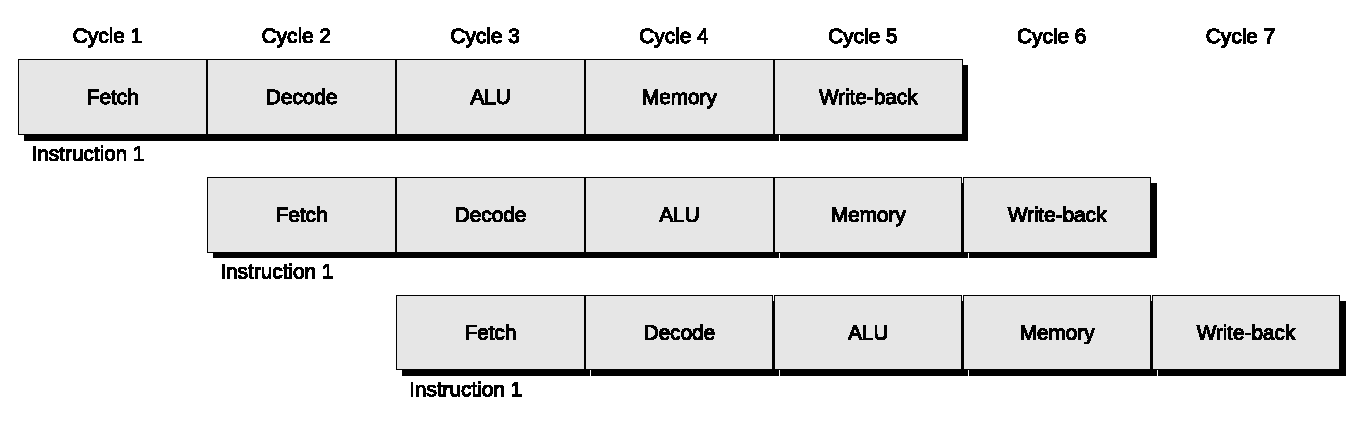
\includegraphics[width=\linewidth]{pictures/pipeline_ex.eps}
   \caption{Five-Deep Single-Completion Pipeline.}
   \label{fig:pipeline}
  \end{figure}
  
  \section{Internal General Purpose Registers}
  The current uDLX architecture provide 32 fixed-point general purpose registers: $R_0$ to $R_{15}$. Two of these register have special use for the hardware. One $R_0$ always returns zero, no matter what software attempts to store to it. The other ($R_{15}$) is used by the normal subroutine-calling instruction (Jump and Link) for the return address.
  
  \newpage
  \section{Licenses}
  The uDLX soft core license of usage are free through provided LGPL v3. There is no external IP-core licenses related to uDLX core system development.
  
% \bibliographystyle{ieeetr}
% \bibliography{ipprocess}

\end{document}
